\chapter{对太阳系内小天体受木星摄动产生双曲线轨道的讨论}

\section{方程建立与求解}

\subsection{建立圆形限制性三体系统}

以太阳、木星为主天体,小天体为第三体建立圆形限制性三体系统。我们作以下的无量纲化规定:
\begin{align}
    m_{\bigodot}+m_J=1
    \\m_J=\mu
    \\a_J=1
    \\n_J=1
    \\G=1
\end{align}
其中,$m_{\bigodot}$与$m_J$为太阳、木星的质量,$a$为木星绕太阳作椭圆运动的半长轴,$n_J$为木星的平运动角频率,$G$为万有引力常量。木星绕太阳的椭圆轨道偏心率较小,因此我们不妨先假定木星绕太阳的轨道为圆,在此假定下分析小天体的运动情况。

转动参考系下圆形限制性三体系统的雅可比积分:
\begin{align}
    \frac{1}{2}\left( \dot{x}^2+\dot{y}^2+\dot{z}^2\right)-\frac{1}{2}\left( x^2+y^2\right)-\frac{1-\mu}{r_1}-\frac{\mu}{r_2}=-\frac{1}{2}C_J
\end{align}
其中$1-\mu$、$\mu$为太阳和木星的质量,$C_J$为雅可比常量。

转动参考系下第三体的Hill曲面:
\begin{align}
    \frac{1}{2}\left( x^2+y^2\right)+\frac{1-\mu}{r_1}+\frac{\mu}{r_2}-\frac{1}{2}C_J=0
\end{align}

根据雅可比常量的不同取值,运动允许区的几何性质会发生改变,因此雅可比常量与各秤动点对应雅可比常量的大小关系可用作研究不同轨道性质的判据。

\subsection{求解运动微分方程组}

转动参考系下的第三体运动微分方程组:
\begin{align}
    \dot{x}&=v_x
    \\\dot{y}&=v_y
    \\\dot{z}&=v_z
    \\\dot{v_x}&=2v_y+\frac{\partial \Omega}{\partial x}
    \\\dot{v_y}&=-2v_x+\frac{\partial \Omega}{\partial y}
    \\\dot{v_z}&=\frac{\partial \Omega}{\partial z}
    \\\Omega&=\frac{1}{2}\left( x^2+y^2\right)+\frac{1-\mu}{r_1}+\frac{\mu}{r_2}
    \\r_1&=\sqrt{(x+\mu)^2+y^2+z^2}
    \\r_2&=\sqrt{(x+\mu-1)^2+y^2+z^2}
\end{align}

给定转动参考系下的初始坐标、速度,通过求解微分方程组即可得到某一时刻小天体在转动参考系下的的坐标、速度。如果给定的初始速度是惯性参考系下的表示,则需要将其转换为转动参考系下的表示:
\begin{align}
    v_{x0}&=v_{\xi0}+y_0
    \\v_{y0}&=v_{\eta0}-x_0
    \\v_{z0}&=v_{\zeta0}
\end{align}
其中$v_{\xi0}$、$v_{\eta0}$、$v_{\zeta0}$是惯性参考系下的初始速度分量。

\subsection{坐标转换}

由于所得结果是转动参考系下的表示,需要进行转动参考系与惯性参考系的转换:
\begin{align}
    \boldsymbol{r}&=R(f)\boldsymbol{r'}
    \\\dot{\boldsymbol{r}}&=\dot{R}(f)\boldsymbol{r'}+R(f)\dot{\boldsymbol{r'}}
    \\R(f)&=
        \left(
        \begin{matrix}
        \cos t & -\sin t & 0\\
        \sin t & \cos t & 0\\
        0 & 0 & 1
        \end{matrix}
    \right)
    \\\dot{R}(f)&=
        \begin{pmatrix}
        -\sin t & -\cos t & 0\\
        \cos t & -\sin t & 0\\
        0 & 0 & 0
        \end{pmatrix}
\end{align}
其中$\boldsymbol{r'}$、$\dot{\boldsymbol{r'}}$为转动参考系下的坐标、速度,$\boldsymbol{r}$、$\dot{\boldsymbol{r}}$为惯性参考系下的坐标、速度。

转换结果:
\begin{align}
   \xi&=x\cos t-y\sin t
    \\\eta&=x\sin t+y\cos t
    \\\zeta&=z
    \\\dot{\xi}&=-x\sin t-y\cos t+\dot{x}\cos t-\dot{y}\sin t
    \\\dot{\eta}&=x\cos t-y\sin t+\dot{x}\sin t+\dot{y}\cos t
    \\\dot{\zeta}&=\dot{z}
\end{align}

\subsection{求解吻切轨道偏心率}

通过二体运动坐标、速度与轨道根数的转换,即可得到吻切轨道的偏心率:
\begin{align}
    \boldsymbol{r}&=r(\cos f)\boldsymbol{P}+r(\sin f)\boldsymbol{Q}
    \\\dot{\boldsymbol{r}}&=-\frac{h}{p}(\sin f)\boldsymbol{P}+\frac{h}{p}(e+\cos f)\boldsymbol{Q}
    \\r&=\frac{a\left| e^2-1\right|}{1+e\cos f}
    \\\frac{h}{p}&=\sqrt{\frac{1-\mu}{p}}=\sqrt{\frac{1-\mu}{a\left| e^2-1\right|}}
    \\\boldsymbol{P}&=
        \left(
        \begin{array}{cc}
        \cos\Omega\cos\omega-\sin\Omega\sin\omega\cos i\\
        \sin\Omega\cos\omega+\cos\Omega\sin\omega\cos i\\
        \sin\Omega\sin i
        \end{array}
        \right)
    \\\boldsymbol{Q}&=
        \left(
        \begin{array}{cc}
        -\cos\Omega\sin\omega-\sin\Omega\cos\omega\cos i\\
        -\sin\Omega\sin\omega+\cos\Omega\cos\omega\cos i\\
        \cos\Omega\sin i
        \end{array}
        \right)
\end{align}

求解六个吻切根数的完整方程组:
\begin{align}
    \xi=&\frac{a\left| e^2-1\right|}{1+e\cos f}[\cos f(\cos\Omega\cos\omega-\sin\Omega\sin\omega\cos i)
    \notag\\&+\sin f(-\cos\Omega\sin\omega-\sin\Omega\cos\omega\cos i)]
    \\\eta=&\frac{a\left| e^2-1\right|}{1+e\cos f}[\cos f(\sin\Omega\cos\omega+\cos\Omega\sin\omega\cos i)
    \notag\\&+\sin f(-\sin\Omega\sin\omega+\cos\Omega\cos\omega\cos i)]
    \\\zeta=&\frac{a\left| e^2-1\right|}{1+e\cos f}[\cos f\sin\Omega\sin i+\sin f\cos\Omega\sin i]
    \\\dot{\xi}=&\sqrt{\frac{1-\mu}{a\left| e^2-1\right|}}-\sin f(\cos\Omega\cos\omega-\sin\Omega\sin\omega\cos i)
    \notag\\&+(e+\cos f)(-\cos\Omega\sin\omega-\sin\Omega\cos\omega\cos i)
    \\\dot{\eta}=&\sqrt{\frac{1-\mu}{a\left| e^2-1\right|}}[-\sin f(\sin\Omega\cos\omega+\cos\Omega\sin\omega\cos i)
    \notag\\&+(e+\cos f)(-\sin\Omega\sin\omega+\cos\Omega\cos\omega\cos i)]
    \\\dot{\zeta}=&\sqrt{\frac{1-\mu}{a\left| e^2-1\right|}}[-\sin f\sin\Omega\sin i+(e+\cos f)\cos\Omega\sin i]
\end{align}
由于我们将重点放在研究吻切轨道的偏心率上,因此可以不必求解其余的吻切根数。

令:
\begin{align}
    p&=a\left| e^2-1\right|
    \\\theta&=f+\omega
\end{align}
同时,取$i=\Omega=0$,将任一时刻的坐标与速度矢量置于$xOy$平面,且小天体位于$x$轴上。

于是,方程组简化为:
\begin{align}
    r&=\frac{p\cos\theta}{1+e\cos(\theta-\omega)}
    \\0&=\frac{p\sin\theta}{1+e\cos(\theta-\omega)}
    \\v\cos\alpha&=-\sqrt{\frac{1-\mu}{p}}(\sin\theta+e\sin\omega)
    \\v\sqrt{1-\cos^2\alpha}&=\sqrt{\frac{1-\mu}{p}}(\cos\theta+e\cos\omega)
\end{align}

其中:
\begin{align}
    r&=\sqrt{\xi^2+\eta^2+\zeta^2}
    \\v&=\sqrt{\dot{\xi}^2+\dot{\eta}^2+\dot{\zeta}^2}
    \\\cos\alpha&=\frac{\xi\dot{\xi}+\eta\dot{\eta}+\zeta\dot{\zeta}}{\sqrt{\xi^2+\eta^2+\zeta^2}\sqrt{\dot{\xi}^2+\dot{\eta}^2+\dot{\zeta}^2}}
\end{align}
解该方程组即可得到吻切轨道的偏心率。

\section{小天体受木星摄动飞离太阳系的条件}

\subsection{无返假设下的初始条件}

假设一小天体初始时刻绕太阳运动的轨道偏心率$e<1$,则其轨道能量满足关系:
\begin{align}
    \frac{1}{2}v^2-\frac{1-\mu}{r_1}<0
\end{align}

而经木星摄动后飞离太阳系,假设其不再返回,则其在转动参考系中的能量为正:
\begin{align}
    \frac{1}{2}\left(\dot{x}^2+\dot{y}^2+\dot{z}^2\right)-\frac{1}{2}\left( x^2+y^2\right)-\frac{1-\mu}{r_1}-\frac{\mu}{r_2}>0
\end{align}
需要说明,在惯性参考系中,小天体经过木星摄动后若能量增加,则木星与太阳的能量相应减少(可理解为木星、太阳对小天体做功),而该减少量相对木星与太阳的能量可忽略不计,因此无法通过分析惯性参考系中的能量情况判定小天体的最终轨道。

将上述两式统一用惯性参考系表示,即得到运动条件的限制:
\begin{align}
    &\frac{1}{2}\left(\dot{\xi}^2+\dot{\eta}^2+\dot{\zeta}^2\right)-\frac{1-\mu}{\sqrt{(\xi+\mu)^2+\eta^2+\zeta^2}}<0
    \\&\frac{1}{2}[(\dot{\xi}+\eta)^2+(\dot{\eta}-\xi)^2+\dot{\zeta}^2]-\frac{1}{2}\left(\xi^2+\eta^2\right)-\frac{1-\mu}{\sqrt{(\xi+\mu)^2+\eta^2+\zeta^2}}
    \notag\\&-\frac{\mu}{\sqrt{(\xi+\mu-1)^2+\eta^2+\zeta^2}}>0
\end{align}
只需找到满足上述条件的初始值集,即可获得飞离太阳系的小天体轨道。

\subsection{相对静止}

假设小天体初始时刻相对木星静止,则初始条件为:
\begin{align}
    &\frac{1}{2}\left(\eta_0^2+\xi_0^2\right)-\frac{1-\mu}{\sqrt{(\xi_0+\mu)^2+\eta_0^2+\zeta_0^2}}<0
    \\&-\frac{1}{2}\left(\xi_0^2+\eta_0^2\right)-\frac{1-\mu}{\sqrt{(\xi_0+\mu)^2+\eta_0^2+\zeta_0^2}}-\frac{\mu}{\sqrt{(\xi_0+\mu-1)^2+\eta_0^2+\zeta_0^2}}>0\label{energy_static}
\end{align}
显然式(\ref{energy_static})的条件是无法满足的,因此若小天体初始时刻相对木星静止,则其无法逃逸至无穷远处。

\subsection{$\xi O\eta$平面限制情况讨论}

令$\zeta=\dot{\zeta}\equiv0$,轨道能量条件简化为:
\begin{align}
    &\frac{1}{2}\left(\dot{\xi}^2+\dot{\eta}^2\right)-\frac{1-\mu}{\sqrt{(\xi+\mu)^2+\eta^2}}<0
    \\&\frac{1}{2}[(\dot{\xi}+\eta)^2+(\dot{\eta}-\xi)^2]-\frac{1}{2}\left(\xi^2+\eta^2\right)-\frac{1-\mu}{\sqrt{(\xi+\mu)^2+\eta^2}}-\frac{\mu}{\sqrt{(\xi+\mu-1)^2+\eta^2}}>0
\end{align}

对应初始条件限制为:
\begin{align}
    &\frac{1}{2}\left(v_{\xi0}^2+v_{\eta0}^2\right)-\frac{1-\mu}{\sqrt{(\xi_0+\mu)^2+\eta_0^2}}<0
    \\&\frac{1}{2}\left[(v_{\xi0}+\eta_0)^2+(v_{\eta0}-\xi_0)^2\right]-\frac{1}{2}\left(\xi_0^2+\eta_0^2\right)-\frac{1-\mu}{\sqrt{(\xi_0+\mu)^2+\eta_0^2}}
    \notag\\&-\frac{\mu}{\sqrt{(\xi_0+\mu-1)^2+\eta_0^2}}>0
\end{align}
以上不等式组包含四个独立变量,我们可以限制其中两个变量的初始值,讨论特殊情况下不等式组的简化结果。

\subsubsection{$\xi_0=1\quad v_{\xi0}=0$}
初始条件简化为:
\begin{align}
    &\frac{1}{2}v_{\eta0}^2-\frac{1-\mu}{\sqrt{(1+\mu)^2+\eta_0^2}}<0\label{energy_11}
    \\&\frac{1}{2}(v_{\eta0}-1)^2-\frac{1-\mu}{\sqrt{(1+\mu)^2+\eta_0^2}}-\frac{\mu}{\sqrt{\mu^2+\eta_0^2}}-\frac{1}{2}>0\label{energy_12}
\end{align}

解以上不等式组可知,当$0<\mu<\frac{1}{3}$时:
\begin{align}
    v_{\eta11}<v_{\eta0}<v_{\eta12}\label{v_eta_1}
\end{align}

其中:
    \begin{align}
    &\left(\eta_0^2+\mu^2+2\mu+1\right)v_{\eta11}^4-4\mu^2+8\mu-4=0
    \\
    &\left(\eta_0^8+4 \mu ^2 \eta_0^6+4 \mu  \eta_0^6+2 \eta_0^6+6 \mu ^4 \eta_0^4+12 \mu ^3 \eta_0^4+10 \mu ^2 \eta_0^4+4 \mu  \eta_0^4+\eta_0^4+4 \mu ^6 \eta_0^2+12 \mu ^5 \eta_0^2\right.
    \notag\\
    &\left.+14 \mu ^4 \eta_0^2+8 \mu ^3 \eta_0^2+2 \mu ^2 \eta_0^2+\mu ^8+4 \mu ^7+6 \mu ^6+4 \mu ^5+\mu ^4\right) v_{\eta12}^8
    \notag\\
    &+\left(-8 \eta_0^8-32 \mu ^2 \eta_0^6-32 \mu  \eta_0^6-16 \eta_0^6-48 \mu ^4 \eta_0^4-96 \mu ^3 \eta_0^4-80 \mu ^2 \eta_0^4-32 \mu  \eta_0^4-8 \eta_0^4\right.
    \notag\\
    &-32 \mu ^6 \eta_0^2-96 \mu ^5 \eta_0^2-112 \mu ^4 \eta_0^2-64 \mu ^3 \eta_0^2-16 \mu ^2 \eta_0^2-8 \mu ^8-32 \mu ^7-48 \mu ^6-32 \mu ^5
    \notag\\
    &\left.-8 \mu ^4\right) v_{\eta12}^7
    \notag\\
    &+\left(24 \eta_0^8+96 \mu ^2 \eta_0^4+288 \mu ^3 \eta_0^4+240 \mu ^2 \eta_0^4+96 \mu  \eta_0^4+24 \eta_0^4+96 \mu ^6 \eta_0^2+288 \mu ^5 \eta_0^2+336 \mu ^4\right.
    \notag\\
    &\left. \eta_0^2+192 \mu ^3 \eta_0^2+48 \mu ^2 \eta_0^2+24 \mu ^8+96 \mu ^7+144 \mu ^6+96 \mu ^5+24 \mu ^4\right) v_{\eta12}^6
    \notag\\
    &+\left(-32 \eta_0^8-128 \mu ^2 \eta_0^6-128 \mu  \eta_0^6-64 \eta_0^6-192 \mu ^4 \eta_0^4-384 \mu ^3 \eta_0^4-320 \mu ^2 \eta_0^4-128 \mu  \eta_0^4\right.
    \notag\\
    &-32 \eta_0^4-128 \mu ^6 \eta_0^2-384 \mu ^5 \eta_0^2-448 \mu ^4 \eta_0^2-256 \mu ^3 \eta_0^2-64 \mu ^2 \eta_0^2-32 \mu ^8-128 \mu ^7
    \notag\\
    &\left.-192 \mu ^6-128 \mu ^5-32 \mu ^4\right) v_{\eta12}^5
    \notag\\
    &+\left(16 \eta_0^8+48 \mu ^2 \eta_0^6+80 \mu  \eta_0^6+24 \eta_0^6+48 \mu ^4 \eta_0^4+192 \mu ^3 \eta_0^4+144 \mu ^2 \eta_0^4+64 \mu  \eta_0^4+8 \eta_0^4\right.
    \notag\\
    &\left.+16 \mu ^6 \eta_0^2+144 \mu ^5 \eta_0^2+184 \mu ^4 \eta_0^2+96 \mu ^3 \eta_0^2+8 \mu ^2 \eta_0^2+32 \mu ^7+64 \mu ^6+32 \mu ^5\right) v_{\eta12}^4
    \notag\\
    &+\left(64 \mu ^8+128 \mu ^7+192 \eta_0^2 \mu ^6+128 \mu ^6+192 \eta_0^2 \mu ^5+128 \mu ^5+192 \eta_0^4 \mu ^4+160 \eta_0^2 \mu ^4+64 \mu ^4\right.
    \notag\\
    &\left.+128 \eta_0^2 \mu ^3+64 \eta_0^6 \mu ^2+64 \eta_0^4 \mu ^2+96 \eta_0^2 \mu ^2-64 \eta_0^6 \mu +32 \eta_0^6+32 \eta_0^4\right) v_{\eta12}^3
    \notag\\
    &+\left(-64 \mu ^8-128 \mu ^7-192 \eta_0^2 \mu ^6-128 \mu ^6-192 \eta_0^2 \mu ^5-128 \mu ^5-192 \eta_0^4 \mu ^4-160 \eta_0^2 \mu ^4-64 \mu ^4\right.
    \notag\\
    &\left.-128 \eta_0^2 \mu ^3-64 \eta_0^6 \mu ^2-64 \eta_0^4 \mu ^2-96 \eta_0^2 \mu ^2+64 \eta_0^6 \mu -32 \eta_0^6-32 \eta_0^4\right) v_{\eta12}^2
    \notag\\
    &+256 \mu ^6+16 \eta_0^4+256 \eta_0^2 \mu ^4-128 \eta_0^2 \mu ^3+64 \eta_0^4 \mu ^2-64 \eta_0^4 \mu=0
\end{align}
当$\frac{1}{3}\leq\mu\leq\frac{1}{2}$时,$\eta_0$须满足$|\eta_0|>\sqrt{\frac{-7 \mu ^4+16 \mu ^3-8 \mu ^2}{8 (\mu -1)^2}+\frac{1}{8} \sqrt{\frac{\mu ^8+32 \mu ^7-48 \mu ^6+16 \mu ^4}{(\mu -1)^4}}}$,$v_{\eta0}$的要求同式(\ref{v_eta_1})。
代入木星质量$\mu=0.000953391$,可得到$\eta_0-v_{\eta0}$的允许范围图像:

\begin{figure}[h]
    \centering
    \subfigure[]{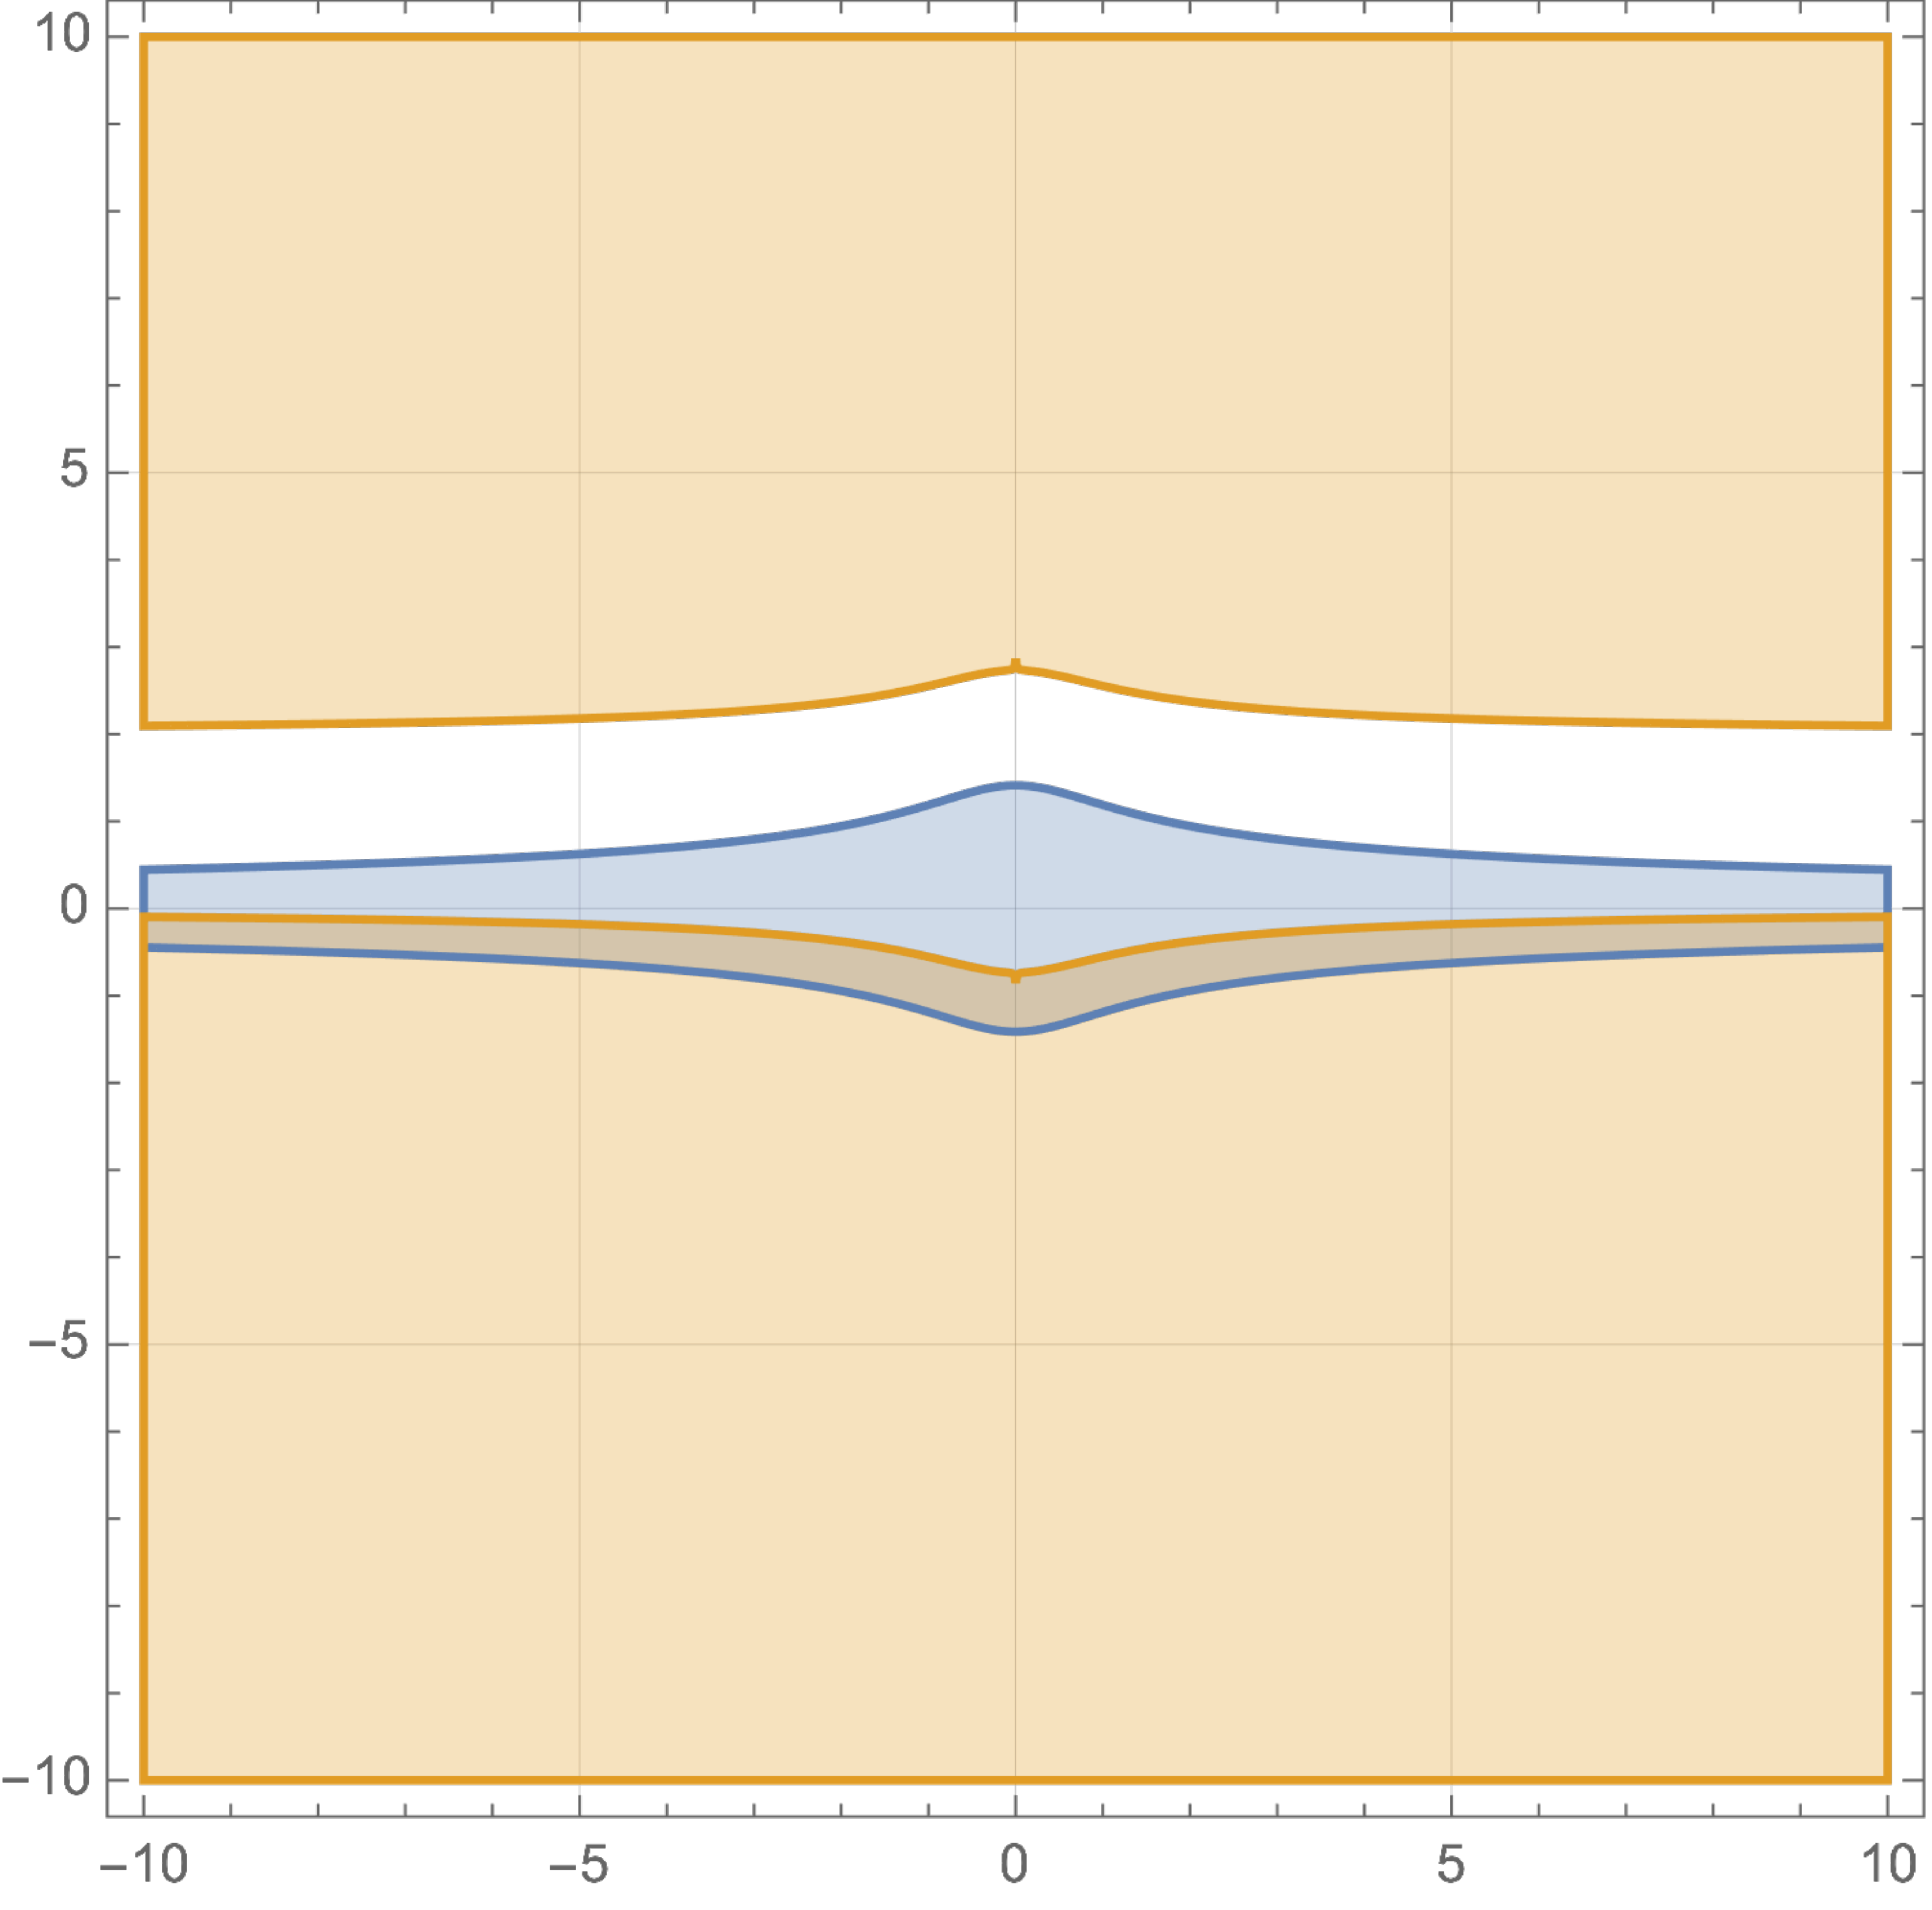
\includegraphics[width=0.45\textwidth]{figures/chapter4/特殊情况1.1.png}}
    \subfigure[]{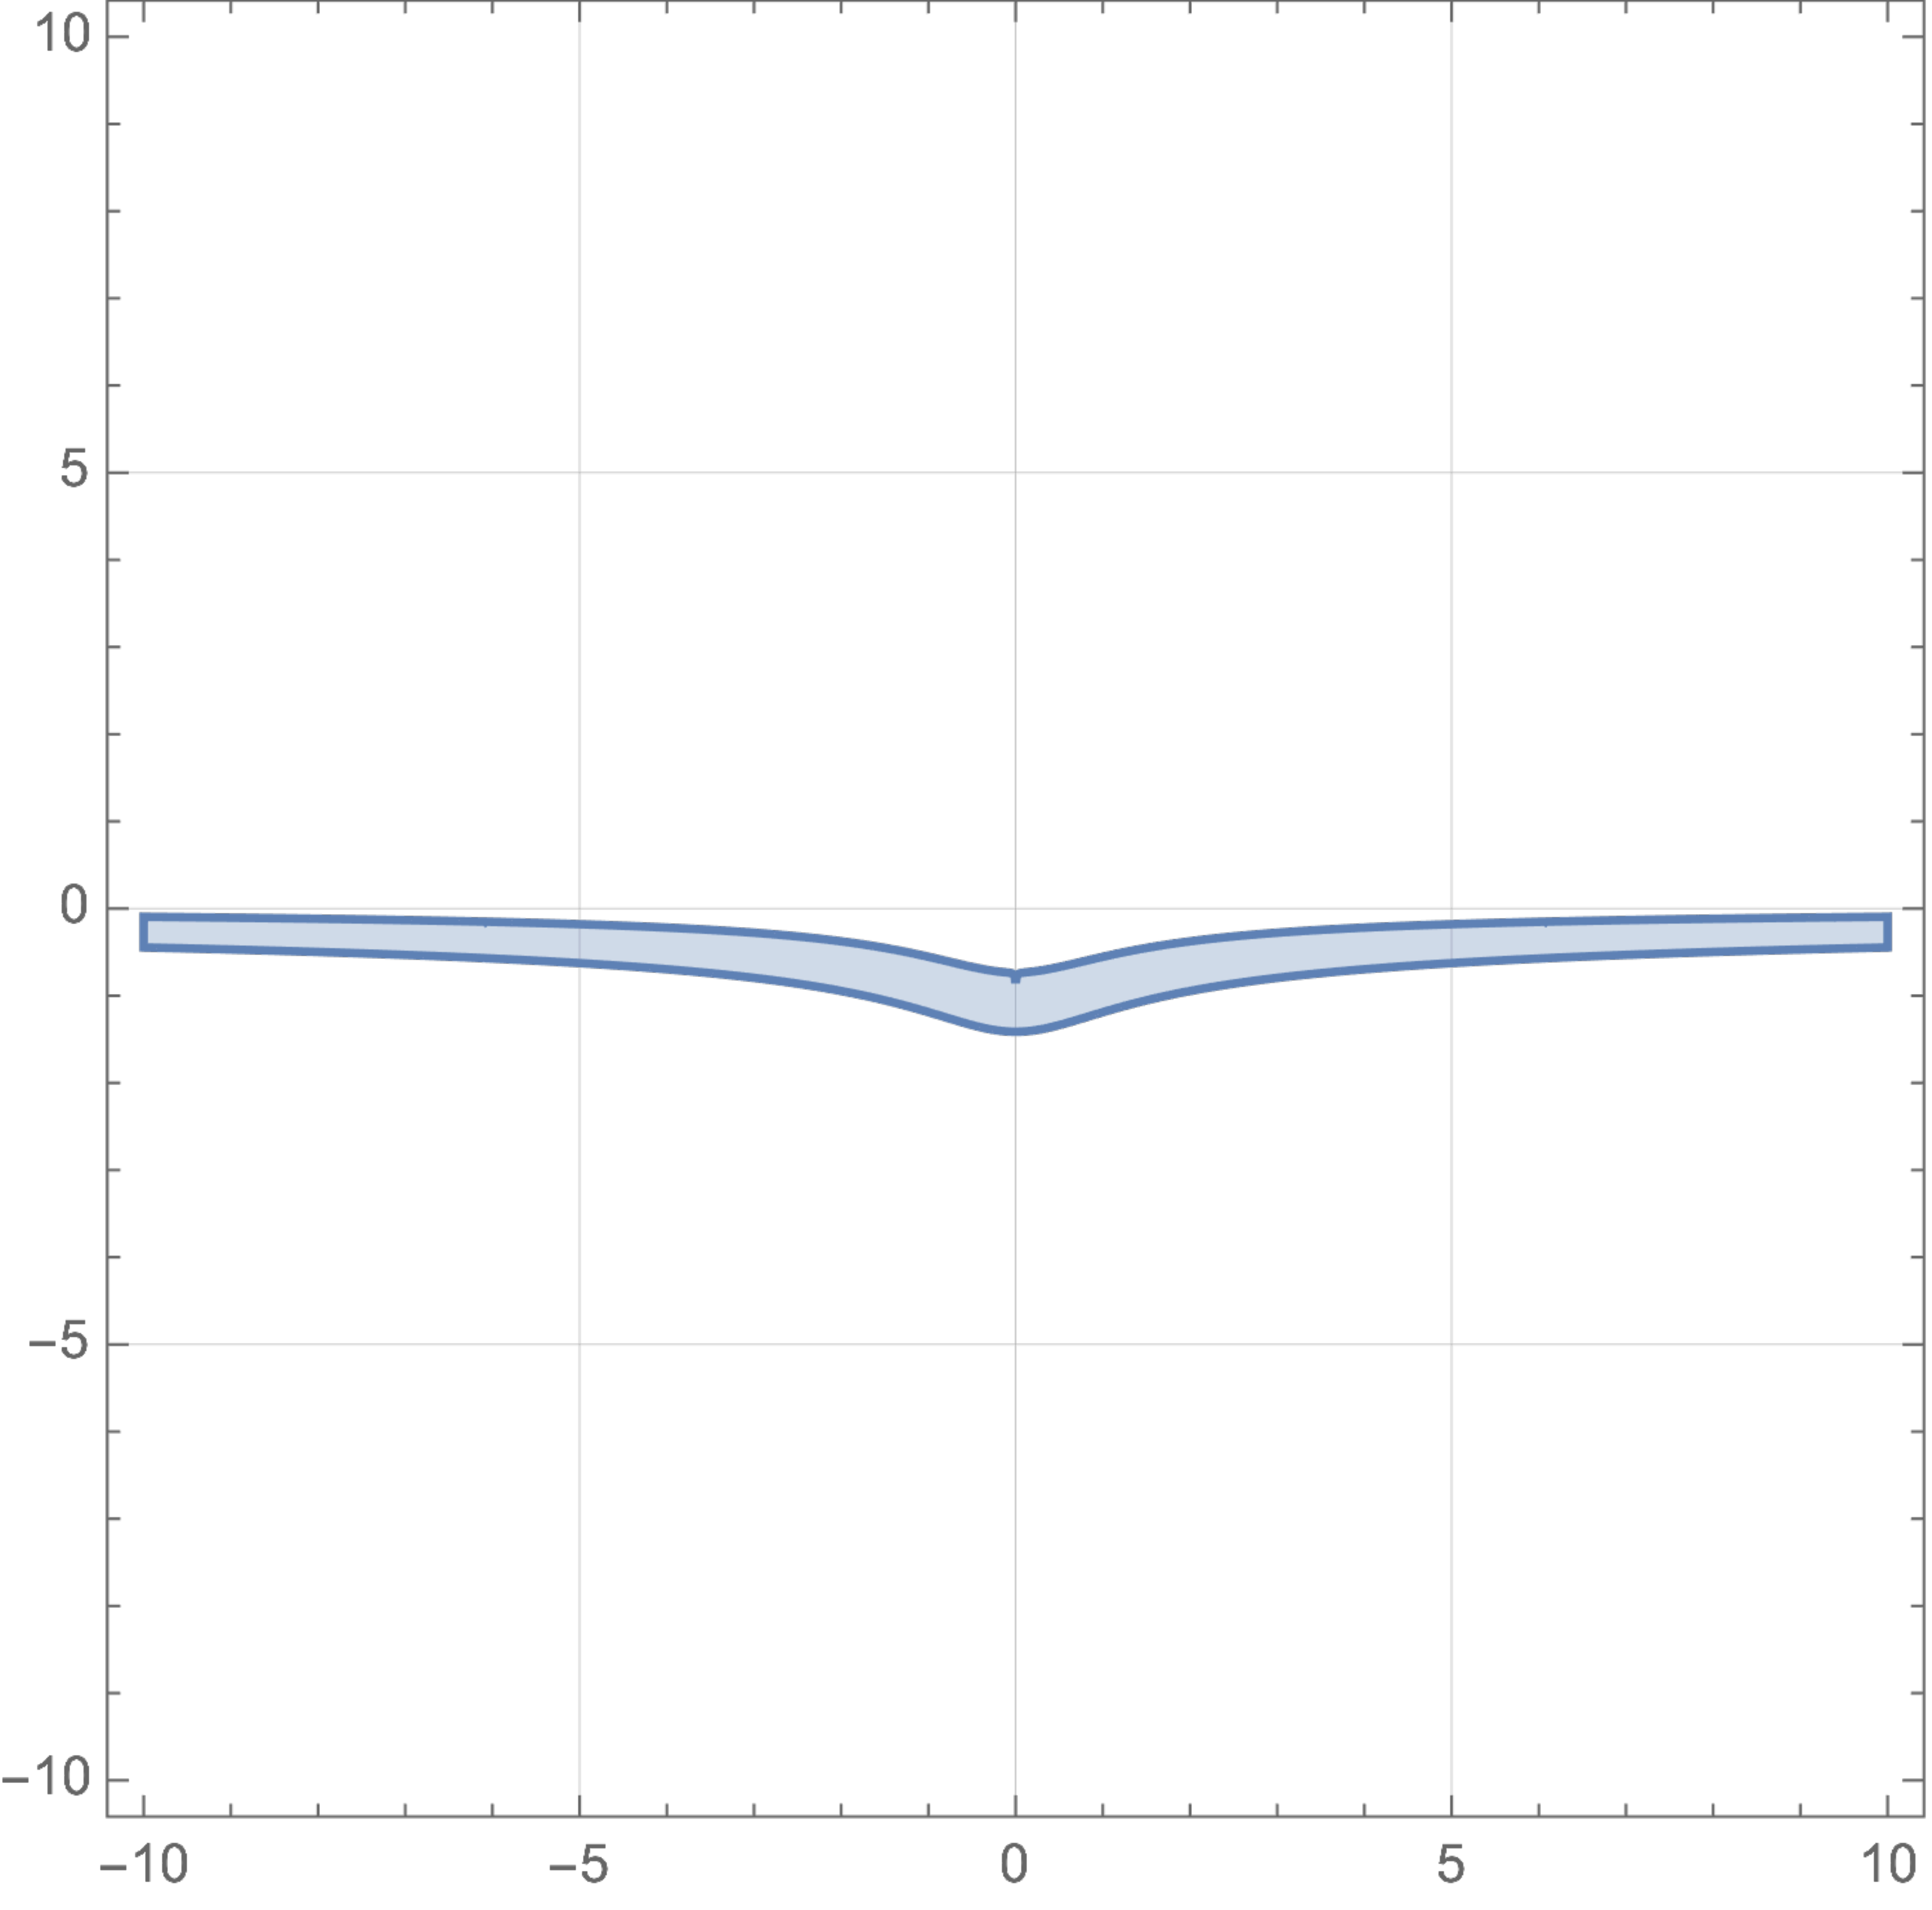
\includegraphics[width=0.45\textwidth]{figures/chapter4/特殊情况1.2.png}}
\end{figure}
\begin{figure}[h]
    \centering
    \subfigure[]{\includegraphics[width=0.45\textwidth]{figures/chapter4/特殊情况1.3.png}}
    \subfigure[]{\includegraphics[width=0.45\textwidth]{figures/chapter4/特殊情况1.4.png}}
    \caption{$\eta_0-v_{\eta0}$的允许范围,$\mathrm{( a)}$中显示了不等式$\mathrm{(\ref{energy_11})(\ref{energy_12})}$分别对应的区域,$\mathrm{(b)(c)(d)}$中显示了两不等式的重合区域。}
\end{figure}

取$\eta_0=1$,$v_{\eta0}=-1$,绘制小天体在惯性参考系下$T<12000$的轨道:

\begin{figure}[h]
    \centering
    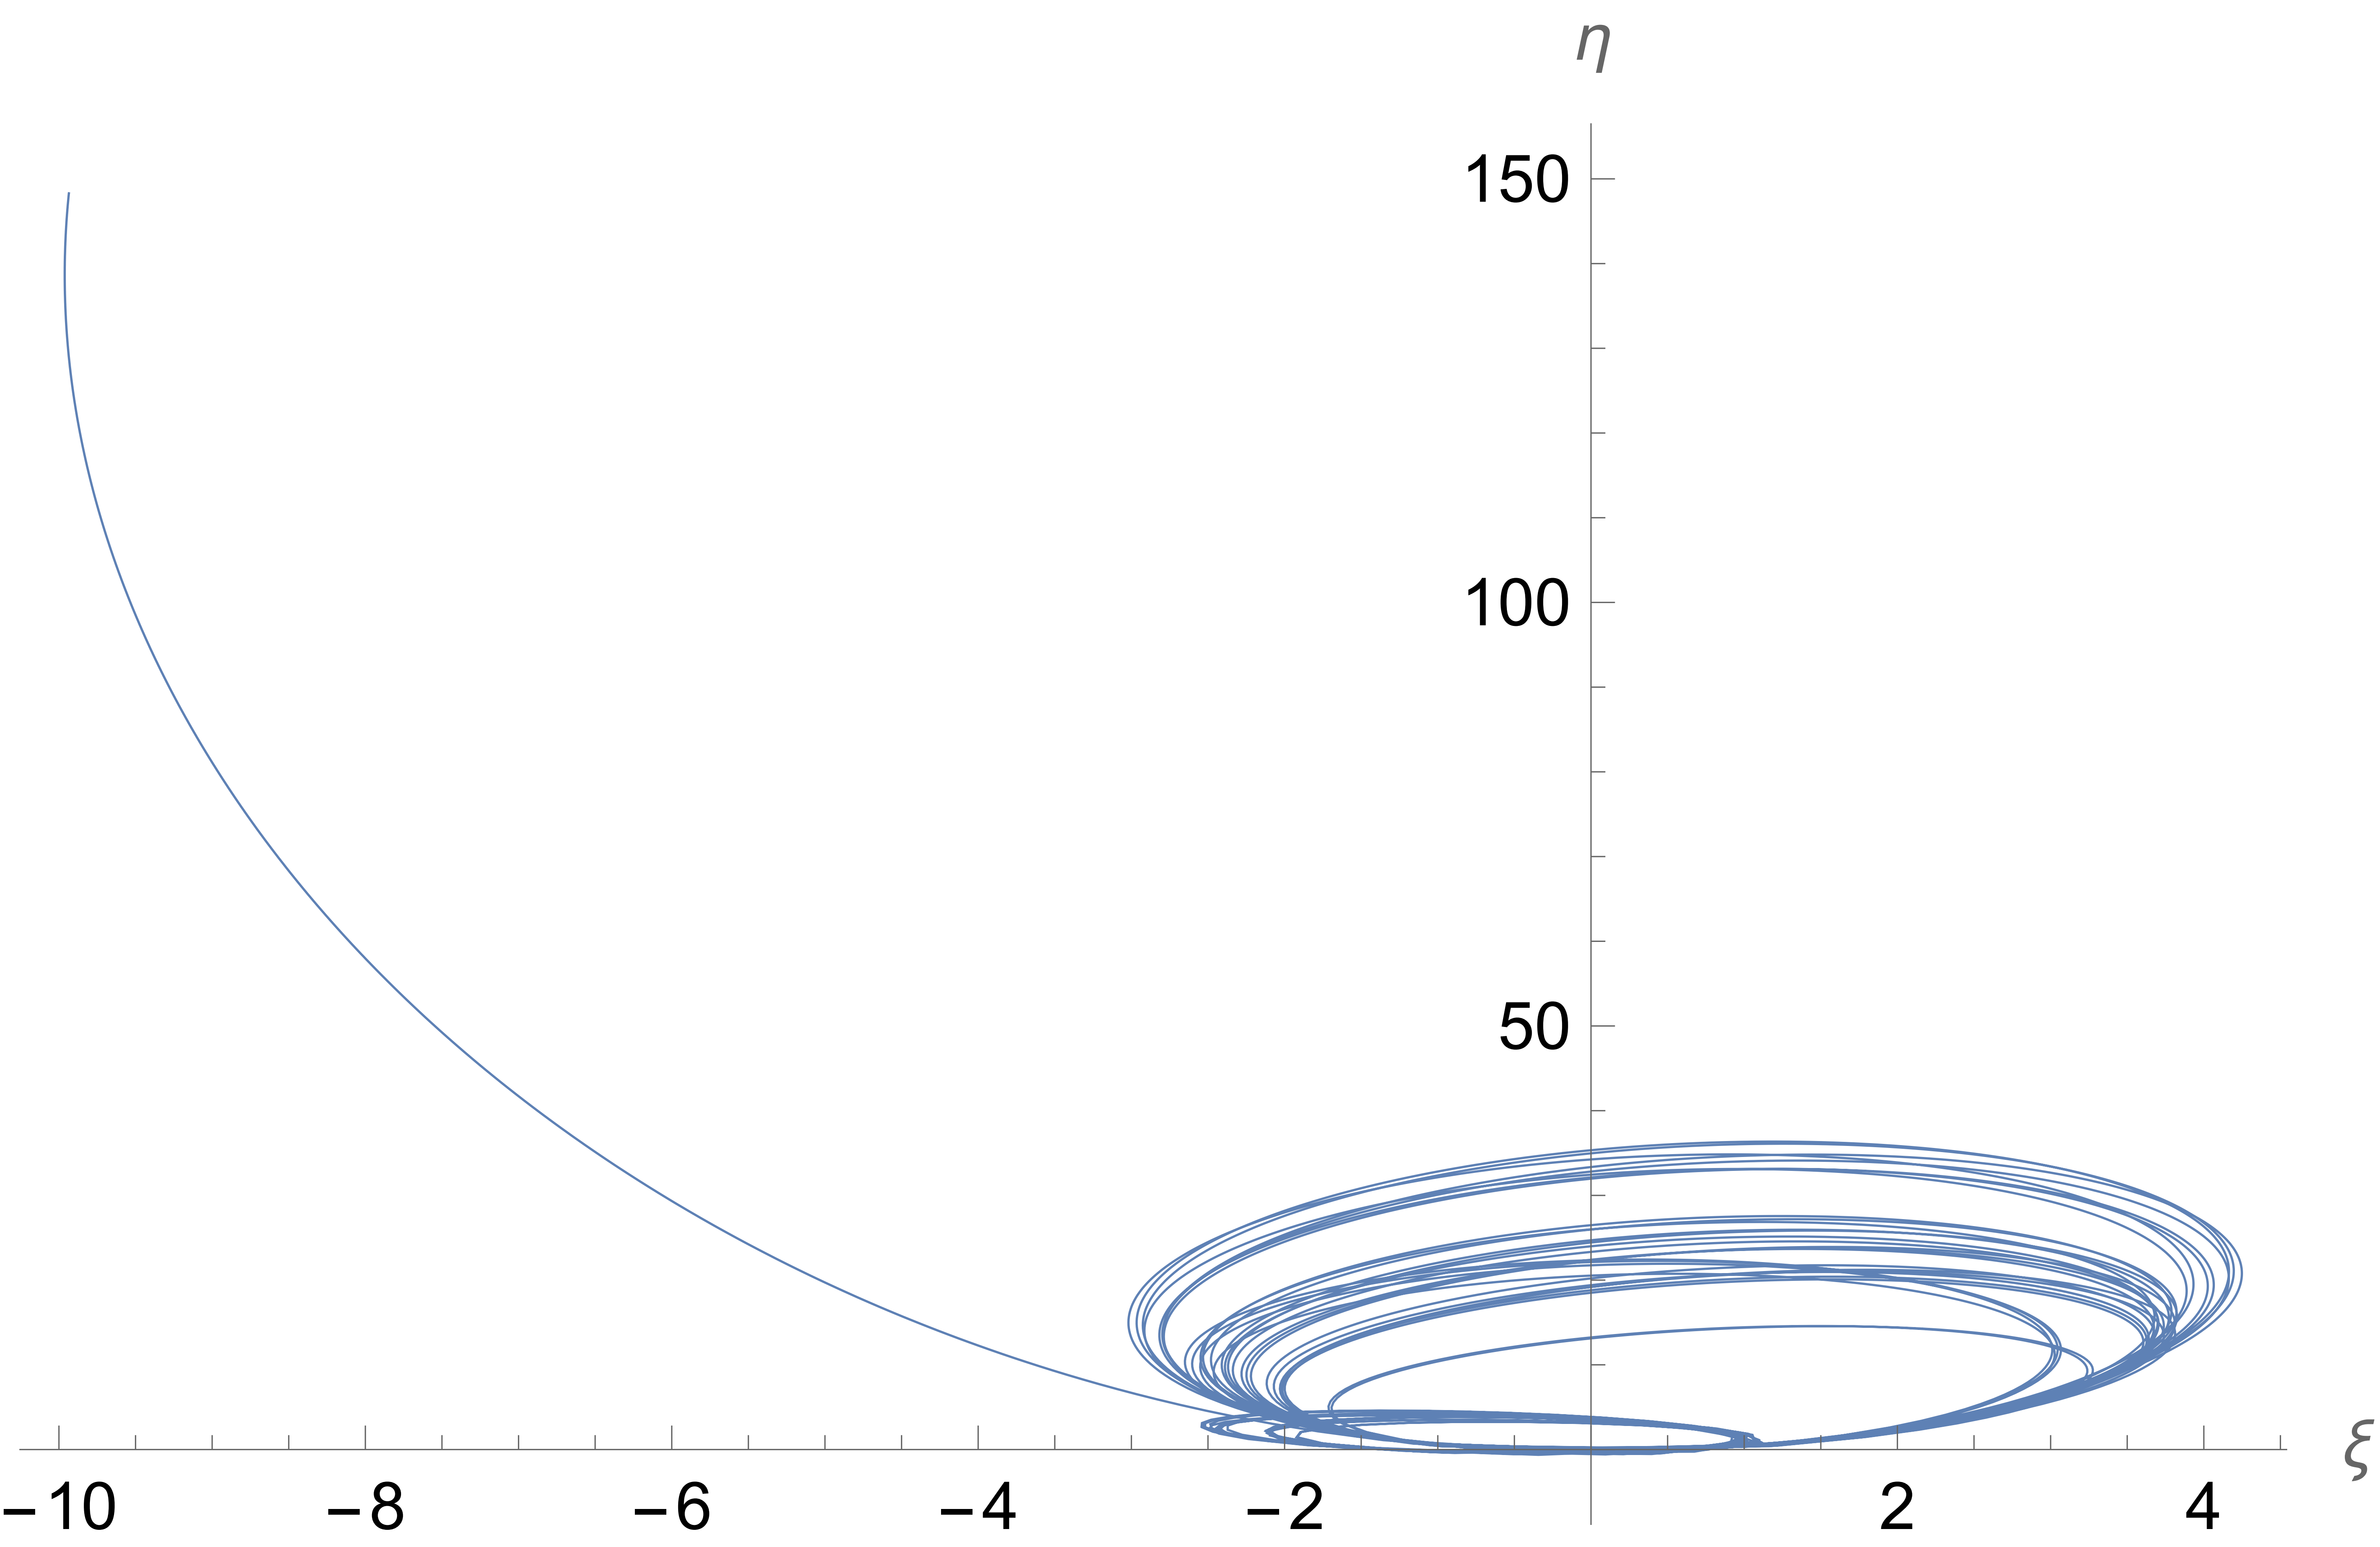
\includegraphics[width=0.8\textwidth]{figures/chapter4/特殊情况1.5.png}
    \caption{小天体在惯性参考系下$T<12000$的轨道}
\end{figure}
可见小天体在运动过程中,其轨道偏心率波动上升,直至产生偏心率极大的轨道从而离开太阳系。

\subsubsection{$\xi_0=1\quad v_{\eta0}=0$}

初始条件简化为:
\begin{align}
    &\frac{1}{2}v_{\xi0}^2-\frac{1-\mu}{\sqrt{(1+\mu)^2+\eta_0^2}}<0
    \\&\frac{1}{2}\left(v_{\xi0}+\eta_0\right)^2-\frac{1}{2}\eta_0^2-\frac{1-\mu}{\sqrt{(1+\mu)^2+\eta_0^2}}-\frac{\mu}{\sqrt{\mu^2+\eta_0^2}}>0
\end{align}

\subsubsection{$\eta_0=0\quad v_{\xi0}=0$}

初始条件简化为:
\begin{align}
    &\frac{1}{2}v_{\eta0}^2-\frac{1-\mu}{|\xi_0+\mu|}<0
    \\&\frac{1}{2}(v_{\eta0}-\xi_0)^2-\frac{1}{2}\xi_0^2-\frac{1-\mu}{|\xi_0+\mu|}-\frac{\mu}{|\xi_0+\mu-1|}>0
\end{align}

解以上不等式组可知,令$\mu_{31}\approx0.236$为方程$64-376x+688x^2-1307x^3+1232x^4-392x^5+64x^6=0$的根,当$0<\mu<\mu_{31}$时,若$\xi _0<-\mu$:

\begin{align}
    \sqrt{\frac{\mu ^2 \xi _0^2+2 \mu  \xi _0^3-\mu  \xi _0^2-4 \mu +\xi _0^4-\xi _0^3-2 \xi _0+2}{\mu ^2+2 \mu  \xi _0-\mu +\xi _0^2-\xi _0}}+\xi _0<v_{\text{$\eta $0}}<\sqrt{\frac{2(\mu -1)}{\mu +\xi _0}}
\end{align}

令方程$ (2 \mu -2)x^4+ \left(4 \mu ^2-8 \mu +4\right)x^3+ \left(2 \mu ^3-6 \mu ^2+6 \mu -2\right)x^2+\mu ^2x+\mu ^3=0$的四个根从小到大分别为$\xi_{31}$、$\xi_{32}$、$\xi_{33}$、$\xi_{34}$。特别地,当$\mu=\frac{2-\sqrt{2}}{4}$时,$\xi_{33}=1-2\mu$。

若$-\mu<\xi _0<\xi_{31}$,则:
\begin{align}
    \sqrt{\frac{\mu ^2 \xi _0^2-4 \mu ^2+2 \mu  \xi _0^3-\mu  \xi _0^2-4 \mu  \xi _0+4 \mu +\xi _0^4-\xi _0^3+2 \xi _0-2}{\mu ^2+2 \mu  \xi _0-\mu +\xi _0^2-\xi _0}}+\xi _0<v_{\text{$\eta $0}}<\sqrt{\frac{2(1-\mu)}{\mu +\xi _0}}
\end{align}

若$\xi_{32}<\xi _0<\xi_{33}$,则:

\begin{align}
    - \sqrt{\frac{2(1-\mu)}{\mu +\xi _0}}<v_{\text{$\eta $0}}<\xi _0-\sqrt{\frac{\mu ^2 \xi _0^2-4 \mu ^2+2 \mu  \xi _0^3-\mu  \xi _0^2-4 \mu  \xi _0+4 \mu +\xi _0^4-\xi _0^3+2 \xi _0-2}{\mu ^2+2 \mu  \xi _0-\mu +\xi _0^2-\xi _0}}
\end{align}

若$\xi _0>\xi_{34}$,则:
\begin{align}
    -\sqrt{\frac{2(1-\mu)}{\mu +\xi _0}}<v_{\text{$\eta $0}}<\xi _0-\sqrt{\frac{\mu ^2 \xi _0^2+2 \mu  \xi _0^3-\mu  \xi _0^2+4 \mu +\xi _0^4-\xi _0^3+2 \xi _0-2}{\mu ^2+2 \mu  \xi _0-\mu +\xi _0^2-\xi _0}}\label{v_eta_34}
\end{align}

当$\mu=\mu_{31}$时,$\xi_{32}=\xi_{33}$,$v_{\eta0}$的第三个可取值区域消失。当$\mu_{31}<\mu\leq\frac{1}{2}$时,$\xi _0<-\mu$与$-\mu<\xi_0<\xi_{31}$的情况与前述相同,$\xi_0>\xi_{32}$时$\v_{\eta0}$的取值同式(\ref{v_eta_34})。

\subsubsection{$\eta_0=0\quad v_{\eta0}=0$}

初始条件简化为:
\begin{align}
    &\frac{1}{2}v_{\xi0}^2-\frac{1-\mu}{|\xi_0+\mu|}<0
    \\&\frac{1}{2}v_{\xi0}^2-\frac{1-\mu}{|\xi_0+\mu|}-\frac{\mu}{|\xi_0+\mu-1|}>0
\end{align}

\subsubsection{$\xi_0=1\quad\eta_0=0$}

初始条件简化为:
\begin{align}
    &\frac{1}{2}\left(v_{\xi0}^2+v_{\eta0}^2\right)-\frac{1-\mu}{1+\mu}<0
    \\&\frac{1}{2}\left[v_{\xi0}^2+(v_{\eta0}-1)^2\right]-\frac{1-\mu}{1+\mu}-\frac{3}{2}>0
\end{align}